% Smart City Technology Investments (recreation of image-012.png)
% Compile with: pdflatex fig-smart-city-investments.tex
\documentclass[border=6pt]{standalone}
\usepackage{pgfplots}
\usetikzlibrary{backgrounds}
\pgfplotsset{compat=1.18}

\definecolor{cardblue}{RGB}{68,114,196}

\begin{document}
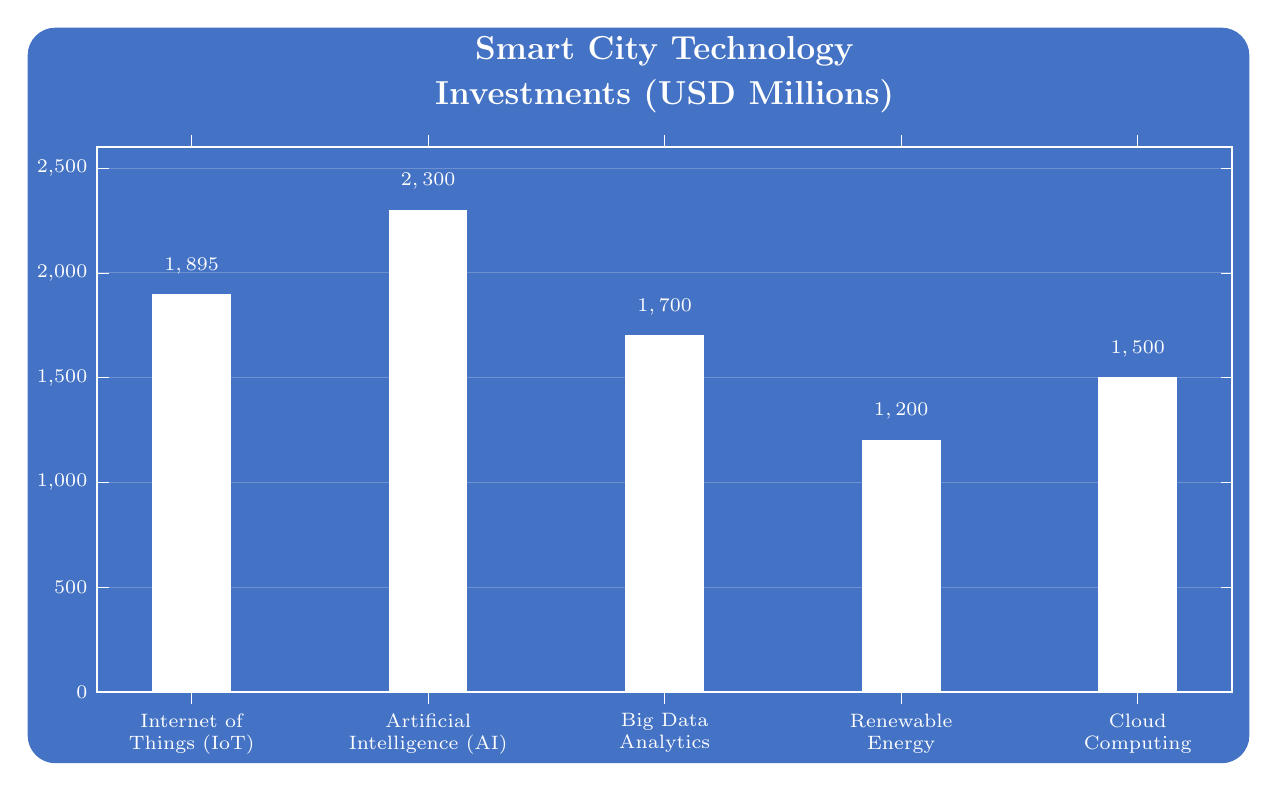
\begin{tikzpicture}
  \begin{axis}[
      width=16cm,
      height=8.5cm,
      title={\textbf{Smart City Technology}\\[2pt]\textbf{Investments (USD Millions)}},
      title style={font=\large, text=white, align=center, yshift=3pt},
      ybar,
      bar width=28pt,
      ymin=0,
      ymax=2600,
      ytick={0,500,1000,1500,2000,2500},
      yticklabels={0,500,1{,}000,1{,}500,2{,}000,2{,}500},
      symbolic x coords={IoT,AI,BigData,Renewable,Cloud},
      xtick=data,
      xticklabels={Internet of\\Things (IoT), Artificial\\Intelligence (AI), Big Data\\Analytics, Renewable\\Energy, Cloud\\Computing},
      xticklabel style={text width=2.6cm, align=center, font=\scriptsize, text=white},
      yticklabel style={font=\scriptsize, text=white},
      ymajorgrids=true,
      grid style={draw=white, opacity=0.22},
      axis line style={draw=white, thick},
      tick style={draw=white},
      axis background/.style={fill=cardblue},
      enlarge x limits=0.10,
      clip=false,
      nodes near coords={\pgfmathprintnumber[fixed,1000 sep={,}]{\pgfplotspointmeta}},
      nodes near coords style={font=\scriptsize\bfseries, text=white, yshift=4pt},
    ]
    \addplot[
      fill=white,
      draw=white,
      bar width=28pt,
    ] coordinates {
      (IoT,1895)
      (AI,2300)
      (BigData,1700)
      (Renewable,1200)
      (Cloud,1500)
    };
  \end{axis}

  % Blue card behind the whole figure (title + labels included)
  \begin{scope}[on background layer]
    \fill[cardblue, rounded corners=10pt]
      (current bounding box.south west) rectangle (current bounding box.north east);
  \end{scope}
\end{tikzpicture}
\end{document}
